%%%%%%%%%%%%%%%%%%%%%%%%%%%%%%%%%%%%%%%%%
% Arsclassica Article
% LaTeX Template
% Version 1.1 (10/6/14)
%
% This template has been downloaded from:
% http://www.LaTeXTemplates.com
%
% Original author:
% Lorenzo Pantieri (http://www.lorenzopantieri.net) with extensive modifications by:
% Vel (vel@latextemplates.com)
% Johan Bos (johan.bos@rug.nl)
% Barbara Plank (bapl@itu.dk)
% 
% License:
% CC BY-NC-SA 3.0 (http://creativecommons.org/licenses/by-nc-sa/3.0/)
%
%%%%%%%%%%%%%%%%%%%%%%%%%%%%%%%%%%%%%%%%%

%----------------------------------------------------------------------------------------
%	PACKAGES AND OTHER DOCUMENT CONFIGURATIONS
%----------------------------------------------------------------------------------------

\documentclass[
10pt, % Main document font size
a4paper, % Paper type
oneside, % One page layout (no page indentation)
headinclude,footinclude, % Extra spacing for the header and footer
%BCOR5mm, % Binding correction
] {book}%


\usepackage{eurosym}
\usepackage{booktabs} % for nice tables with \toprule, \midrule
\usepackage{csvsimple,longtable}
\setcounter{secnumdepth}{5}
%%%%%%%%%%%%%%%%%%%%%%%%%%%%%%%%%%%%%%%%%
% Arsclassica Article
% Structure Specification File
%
% This file has been downloaded from:
% http://www.LaTeXTemplates.com
%
% Original author:
% Lorenzo Pantieri (http://www.lorenzopantieri.net) with extensive modifications by:
% Vel (vel@latextemplates.com)
%
% License:
% CC BY-NC-SA 3.0 (http://creativecommons.org/licenses/by-nc-sa/3.0/)
%
%%%%%%%%%%%%%%%%%%%%%%%%%%%%%%%%%%%%%%%%%

%----------------------------------------------------------------------------------------
%	REQUIRED PACKAGES
%----------------------------------------------------------------------------------------

\usepackage[
%nochapters, % Turn off chapters since this is an article        
beramono, % Use the Bera Mono font for monospaced text (\texttt)
eulermath,% Use the Euler font for mathematics
pdfspacing, % Makes use of pdftex letter spacing capabilities via the microtype package
dottedtoc % Dotted lines leading to the page numbers in the table of contents
]{classicthesis} % The layout is based on the Classic Thesis style


\usepackage{arsclassica} % Modifies the Classic Thesis package

\usepackage[T1]{fontenc} % Use 8-bit encoding that has 256 glyphs

\usepackage[utf8]{inputenc} % Required for including letters with accents

\usepackage{graphicx} % Required for including images

\usepackage{enumitem} % Required for manipulating the whitespace between and within lists

\usepackage{lipsum} % Used for inserting dummy 'Lorem ipsum' text into the template

\usepackage{subfig} % Required for creating figures with multiple parts (subfigures)

\usepackage{amsmath,amssymb,amsthm} % For including math equations, theorems, symbols, etc

\usepackage{varioref} % More descriptive referencing
\usepackage{color}
\usepackage{listings}
\usepackage{setspace}
\usepackage{lscape}
\usepackage[authoryear]{natbib}

%----------------------------------------------------------------------------------------
%	DUTCH SUPPORT
%----------------------------------------------------------------------------------------

%\usepackage[dutch]{babel}    % comment out if you write your thesis in Dutch


%----------------------------------------------------------------------------------------
%	THEOREM STYLES
%---------------------------------------------------------------------------------------

\theoremstyle{definition} % Define theorem styles here based on the definition style (used for definitions and examples)
\newtheorem{definition}{Definition}

\theoremstyle{plain} % Define theorem styles here based on the plain style (used for theorems, lemmas, propositions)
\newtheorem{theorem}{Theorem}

\theoremstyle{remark} % Define theorem styles here based on the remark style (used for remarks and notes)

%----------------------------------------------------------------------------------------
%	HYPERLINKS
%---------------------------------------------------------------------------------------

\hypersetup{
%draft, % Uncomment to remove all links (useful for printing in black and white)
colorlinks=true, breaklinks=true, % bookmarks=true,
bookmarksnumbered,
urlcolor=webbrown, linkcolor=RoyalBlue, citecolor=webgreen, % Link colors
pdftitle={}, % PDF title
pdfauthor={\textcopyright}, % PDF Author
pdfsubject={}, % PDF Subject
pdfkeywords={}, % PDF Keywords
pdfcreator={pdfLaTeX}, % PDF Creator
plainpages=false,
pdfproducer={LaTeX with hyperref and ClassicThesis} % PDF producer
}


\renewcommand{\lstlistingname}{Python code}% Listing -> Python
\renewcommand{\lstlistlistingname}{List of \lstlistingname}% List of Listings -> List of Python
\definecolor{Code}{rgb}{0,0,0}
\definecolor{Decorators}{rgb}{0.5,0.5,0.5}
\definecolor{Numbers}{rgb}{0.5,0,0}
\definecolor{MatchingBrackets}{rgb}{0.25,0.5,0.5}
\definecolor{Keywords}{rgb}{0,0,1}
\definecolor{self}{rgb}{0,0,0}
\definecolor{Strings}{rgb}{0,0.63,0}
\definecolor{Comments}{rgb}{0,0.63,1}
\definecolor{Backquotes}{rgb}{0,0,0}
\definecolor{Classname}{rgb}{0,0,0}
\definecolor{FunctionName}{rgb}{0,0,0}
\definecolor{Operators}{rgb}{0,0,0}
\definecolor{Background}{rgb}{0.98,0.98,0.98}




 
\lstdefinestyle{mystyle}{
numbers=left,
numberstyle=\footnotesize,
numbersep=1em,
xleftmargin=1em,
framextopmargin=10em,
framexbottommargin=2em,
showspaces=false,
showtabs=false,
showstringspaces=false,
frame=l,
tabsize=4,
% Basic
basicstyle=\ttfamily\small\setstretch{1},
backgroundcolor=\color{Background},
language=Python,
% Comments
commentstyle=\color{Comments}\slshape,
% Strings
stringstyle=\color{Strings},
morecomment=[s][\color{Strings}]{"""}{"""},
morecomment=[s][\color{Strings}]{'''}{'''},
% keywords
morekeywords={import,from,class,def,for,while,if,is,in,elif,else,not,and,or,print,break,continue,return,True,False,None,access,as,,del,except,exec,finally,global,import,lambda,pass,print,raise,try,assert},
keywordstyle={\color{Keywords}\bfseries},
% additional keywords
morekeywords={[2]@invariant},
keywordstyle={[2]\color{Decorators}\slshape},
emph={self},
emphstyle={\color{self}\slshape},
captionpos=b, 
}
 
\lstset{style=mystyle}

\def\vl{\\[9pt]}
 % Include the structure.tex file which specified the document structure and layout
\usepackage{makecell}
\usepackage{wrapfig}
\usepackage{graphicx}
\usepackage{float}
\usepackage{chngcntr} %for figure labeling in appendix
\usepackage{longtable}
\usepackage{xurl}
%\usepackage[nottoc,notlot,notlof]{tocbibind}
\usepackage{etoolbox}

%----------------------------------------------------------------------------------------
%	Defined Variables
%----------------------------------------------------------------------------------------



% POLITIFACT VARIABLES 
% ---------------------------------------------------------------------------------------

% Before preprocessing / Removing duplicates
\newcommand{\pltfctBORN}{46749}
% META + Viral videos CLAIMS
\newcommand{\pltfctMETA}{4531}
% pltfctDUPS is all the duplicate claims from our first scrape
\newcommand{\pltfctDUPS}{21785}
% data entries after duplicates and meta/video claims are removed
\newcommand{\pltfctNODUP}{20433}
% Total of integrity date entries (flip-flop)
\newcommand{\pltfctFLIPFLOP}{259}

% POLITIFACT AFTER PREPROCESSING STEPS
% total claims in our data set
\newcommand{\pltfctTOTAL}{20174}
% pltfct topics
\newcommand{\pltfctTOPICS}{145}
% pltfct origins
\newcommand{\pltfctORIGINS}{703}
% "To date" of our date set
\newcommand{\pltfctFROMDATE}{October 1, 2000}
% "from date" of our data set
\newcommand{\pltfctTODATE}{October 4, 2022}
% 75% upper quartiles account from date:
\newcommand{\pltfctMOSTDATE}{March 27, 2012}
% Dem reps labeled in the data set
\newcommand{\pltfctDEMREPS}{13788}
% Dem reps labeled in the data set percent
\newcommand{\pltfctDEMREPSPCT}{68.3\%}
% percentage of the false claims in the total distribution of our date set.
\newcommand{\pltfctFALSECLAIMSPCT}{25.8\%}
% mean length of claims
\newcommand{\pltfctMEANCLAIMLENCHARACTERS}{109}

\newcommand{\pltfctBORN}{46749}% Before preprocessing / Removing duplicate


% DRIVERS 
% ---------------------------------------------------------------------------------------





%----------------------------------------------------------------------------------------
%	HYPHENATION
%----------------------------------------------------------------------------------------

\hyphenation{Fortran hy-phen-ation} % Specify custom hyphenation points in words with dashes where you would like hyphenation to occur, or alternatively, don't put any dashes in a word to stop hyphenation altogether


%----------------------------------------------------------------------------------------
%	TITLE AND AUTHOR(S)
%----------------------------------------------------------------------------------------

\title{\normalfont\spacedallcaps{title}} % The article title

\author{\spacedlowsmallcaps{author}} % The article author(s) - author affiliations need to be specified in the AUTHOR AFFILIATIONS block

\date{} % An optional date to appear under the author(s)

%----------------------------------------------------------------------------------------

\begin{document}

%----------------------------------------------------------------------------------------
%	HEADERS
%----------------------------------------------------------------------------------------

%\renewcommand{\chaptermark}[1]{\markright{\spacedlowsmallcaps{#1}}} % The header for all pages (oneside) or for even pages (twoside)
%\renewcommand{\subsectionmark}[1]{\markright{\thesubsection~#1}} % Uncomment when using the twoside option - this modifies the header on odd pages
%\lehead{\mbox{\llap{\small\thepage\kern1em\color{halfgray} \vline}\color{halfgray}\hspace{0.5em}\rightmark\hfil}} % The header style

\pagestyle{scrheadings} % Enable the headers specified in this block


%----------------------------------------------------------------------------------------
%	TITLE PAGE
%----------------------------------------------------------------------------------------

\hypersetup{pageanchor=false}
\begin{titlepage}
\thispagestyle{empty}
\begin{figure}[h!] %  figure placement: here, top, bottom, or page
\centering

\includegraphics[width=4in]{ITUlogo} 
\end{figure}

\begin{center}
\vspace{30 mm}
\begingroup \linespread{1,75} \selectfont 
\textsc{\LARGE FUGAZI}\\
% \textsc{\Large And this is an optional subtitle}
% Alternative title "How do Politicians Talk about Climate Change?"
[1,5cm]
\endgroup

Laurenz Aisenpreis and Gustav Gyrst\\[2,5cm]

\end{center}
\vfill
\textbf{Research Project}\\  %\textbf{Master thesis}\\
MSc in Software Design\\  
Laurenz Aisenpreis and Gustav Gyrst\\
\\
\today\\
Supervisor: Luca
\end{titlepage}
\hypersetup{pageanchor=true}



%----------------------------------------------------------------------------------------
%	ABSTRACT
%----------------------------------------------------------------------------------------

\pagenumbering{roman}
\chapter*{Abstract}
\markboth{Abstract}{Abstract}
\addcontentsline{toc}{chapter}{Abstract}



%----------------------------------------------------------------------------------------
%	TABLE OF CONTENTS & LISTS OF FIGURES AND TABLES
%----------------------------------------------------------------------------------------
\clearpage
\setcounter{tocdepth}{3} % Set the depth of the table of contents to show sections and subsections only
\tableofcontents % Print the table of contents

\listoffigures % Print the list of figures (optional, only if you have many figures)

\listoftables % Print the list of tables (optional, only if you have many tables)

%\lstlistoflistings



%----------------------------------------------------------------------------------------
%	INTRODUCTION
%----------------------------------------------------------------------------------------

\chapter{Introduction} \label{introduction}


\section{Background}

% Introduction to the topic: what is the phenomenom of fake news, misinformation
% Social Medias impact on the communication and the quality of the news we consume.
% History -> past decade what has happened - why has it gained importance. 
% Why is important to study fake news? (Bot detection, war, political propaganda etc.) 

This paragraph is about highlighting the importance of fighting misinformation and fake news. We discuss the development of fake news in relation to social media. We show different techniques of false information and provide a brief insight into human psychology of decision making.  

\section{Rationale}

We describe in this paragraph the importance of preventing/countering the spread and severity of false information. 
It is important to understand the factors which cause humans to believe misinformation. Here, we apply drivers of misinformation belief to a setting on social media.

%(Profiling Fake News Spreaders) In this work, we provide a methodology to extract factors that are not reliant on currently existing self-reported survey methods [5, 45].

%(Paper: Perceived truth of statements and simulated social media postings: an experimental investigation of source credibility, repeated exposure, and presentation format)

%(people would not willingly share fake news, if they know that they are not true --> source)

% Why study false belief? 
% Why on Twitter?
% Psychology behind endorsing misinformation & sharing misinformation


\section{Definitions and Scope}

In our work, we define "misinformation" as statements - whether they are intentional or not - that are contrary to the available empirical evidence \citep{doi:10.1177/14614448211011451}. We decide on this definition for two reasons.

First, there clearly exists a characteristic difference between misinformation, that is false statements that are well-intentioned, and disinformation, that is spread intentionally. However, we do not distinguish between intent in our study, as psychological drivers influence the false belief formation despite the intent by which the message has been spread \citep{psychological_drivers_misinformation}.

Second, defining misinformation according to its temporal aspect is particularly important in a dynamic and fast-moving context such as social media. What is perceived to be true today, might change with advancements in research \citep{doi:10.1177/14614448211011451}, and will be spread through the internet. Prior beliefs and knowledge, as well as contextual factors  influence the perception of truth and the correction of misinformation. These drivers might change over time.


% \citep{PENNYCOOK2021388}
%We focus here primarily on online content that is presented in the form of news articles. However, false and misleading claims come in many forms, and there are several literatures that are clearly related, but outside the scope of our review (although we will draw some connections throughout). These include work on conspiracy belief [9], superstition [10], rumors [11], bullshit receptivity [12], and misperceptions [13], among others. Furthermore, our focus is on individual examples of misinformation, and not on organized disinformation campaigns (e.g., by the Russian Internet Research Agency, or campaigns relating to global warming or fraud in the 2020 US Presidential Election). 

\section{Research questions}

\begin{itemize}
    %\item RQ1: Which users are more likely to endorse misinformation on Twitter? 
    \item RQ1: How can the psychological drivers of false belief formation be quantified from observational data on social media?
    % How to find misinformation? How to find the people who endorse it? How to quantify the "likelihood"?
    
    % The work for making a "proxy for being in false belief"
    
    %\item RQ2: What psychological drivers influence users to endorse misinformation on Twitter?
    \item RQ2: What is the impact of each psychological driver influencing users forming a false belief?
    
    \item RQ3: Can we use a combination of drivers and claims to predict whether a user forms a false belief about a statement on Twitter?
\end{itemize}

\section{Methodology and Data}

Here we describe our methodology on a high level. 1) Fact-checked claims from Politifact. 2) Twitter users. 3) Engineering of psychological drivers. 4) Examining the relevance and relationships.




\pagenumbering{arabic}




\newpage
\clearpage

\chapter{Theoretical Framework}
\label{chp:theoretical_framework}

\section{Drivers Of Misinformation Belief}
% Introduce the theoretical concept
To investigate factors that lead humans to form or endorse misinformed opinions, we ground our analysis on a reviewed framework that describes psychological drivers of misinformation belief \citep{psychological_drivers_misinformation}. In the past decades, many scholars have focused on examining the effects of single psychological drivers in isolation, such as partisanship \citep{osmundsen2021partisan, baptista2021partisanship, grady2021nevertheless}, the illusory truth effect \citep{wang_illusory_truth, dechene2010truth} or in-group effects \citep{mackie1990processing, wyer2010selective}.  However, people often find themselves influenced by a magnitude of cognitive, social and affective processes when assessing the truth of information \citep{PENNYCOOK2021388}. Hence, we analyze the problem at hand holistically by integrating a magnitude of factors, instead of examining single cognitive and social drivers.

In their framework, \cite{psychological_drivers_misinformation} describe two main categories that drive misinformation belief: \emph{cognitive} and \emph{socio-affective drivers}. Cognitive drivers describe the individual's processing of information, such as how information is encoded in and retrieved from memory. Socio-affective drivers refer to the influence of both external cues and internal beliefs. Social cues, such as the perceived credibility of an information source, can affect the truth judgement of a claim. Likewise, individual's beliefs or values can influence the assessment of a claim depending on whether it's consistent or inconsistent with ones worldview.

As the authors note, not all drivers are guaranteed to be present and of the same relevance, but nevertheless a multitude of factors contribute to false beliefs \citep{psychological_drivers_misinformation}. This complexity would be overlooked by any examination of drivers in isolation.


\section{Capturing False Belief}

% Explain how we define false belief 
The drivers influencing false beliefs, also influence behaviors, such as sharing of misinformation. \cite{psychological_drivers_misinformation} note that the psychological drivers behind sharing misinformation is a highly related area of study. Misinformation might be spread intentionally despite knowing it's false. Research is still at the beginning to disentangle why misinformation is spread and how the interplay between beliefs and behaviors is constituted \citep{van2021political}. Ensuring to capture both the presence of a false belief as well as the rationale of sharing it, requires to combine interviews or surveys with real-world observations on social media. Such a study is either infeasible or limited to a small scale. 

For that reason we focus on individuals who share misinformation in large amounts. We set the act of sharing misinformation frequently to be equivalent to having formed false belief(s).

Especially on Twitter the presence of bots or influence campaigns is known to exist, where the actors are willingly manipulating public opinion by spreading misinformation \citep{stukal2017detecting}. Such actors are not necessarily driven by false beliefs, but rather the sheer motivation to create discord. We address this challenge by defining a heuristic to filter out bots or automated accounts which is described in section XY.

%\section{Quantifying Drivers of Misinformation Belief}
% What we are studying (Twitter, etc)
%In order to assess the interplay between the psychological drivers of misinformation belief and the degree to which a user is endorsing misinformation, we define suitable metrics to quantify each factor. 

%\section{Evaluation of the Importance of Drivers}

\chapter{Related Work}
\label{chp:related_work}

\section{Fake News Detection}
\label{sec:fake_news_detection}

While there are differing opinions on how scholars group the research domain of fake news detection \citep{shu2017datamining, zhou2020survey}. Detecting misinformation (i.e., or fake news) on social media has often been approached with one or a combination of four methodologies \citep{zhou2020survey}: knowledge-based \citep{shu2018userprofiles, shu2020fakenewsnet, mosleh2021elites}, style-based, source-based \citep{grinberg2019partisanship, halberstam2016homophily, lazer2018science, guess2020exposure, osmundsen2021partisan, mosleh2021elites}, propagation-based fake news detection. 

\subsection{Knowledge-based}
\label{subsec:knowledge_based}

\textbf{Knowledge-based} fake news detection focuses on the authenticity of the news shared. The approach thus inherently relies on fact-checking. Fact-checking news can either happen through the wisdom of the crowd, expert annotations of claims, or machine learning classification \citep{zhou2020survey, shu2017datamining}. In table \ref{tbl:fact_checking_services}, six of the well known fact-checking organizations and tools are listed. Several scholars have used these existing fact-checking evaluations as the foundation for their research \citep{shu2018userprofiles, shu2020fakenewsnet, mosleh2021elites}. In particular, \cite{shu2020fakenewsnet} applies Gossipcop and Politifact to create the FakeNewsNet\footnote{The FakeNewsNet is accessible at https://github.com/KaiDMML/FakeNewsNet} and analyze the characteristics of users that spread fake news. \cite{shu2020fakenewsnet} do so by collecting fact-checked news claims from fact-checking organizations (i.e., Gossipcop and Politifact), and querying the claims in the Twitter API to find the users that have tweeted or retweeted these claims. 


% TABLES
\label{app_linear_data_upsample}
%table example
\begin{table}[H]
  \tiny %15
  \begin{center}
  \begin{tabular}{p{1.8cm}|p{1.8cm}|p{3cm}|p{3cm}}
\toprule{} &         Coverage &                                   Topics &                                                 Truth Assessment & Name &                                          &                                                                 \\
\midrule
Politifact            &             U.S. &                                 Politics &                                                       1-6 scale \\
Factcheck             &             U.S. &                                 Politics &                                                          Binary \\
GossipCop             &            U.S.  &           Celebrities, Hollywood, rumors &                                                      0-10 scale \\
Snopes                &             U.S. &                  Politics, social issues &                                      1-5 scale + special labels \\
Reuters               &  European/Global &  Politics, sports, business, environment &  False, partly false, missing context, miscaptioned, misleading \\
Google fact-check API &           Global &                                    Mixed &                                                    Mixed scales \\
\bottomrule
\end{tabular}

  \caption{Overview of six fact-checking services publicly accessible with a wide coverage of topics and geographical scopes, although U.S. Focussed. The last outlined, \emph{Google fact-check API} is a google service that collects fact-checks from a combination of the above fact-checking sites and others.}
  \label{tbl:fact_checking_services}
  \end{center}
\end{table}


% \textbf{style-based fake news detection}... % looking at the content of the style of the content being spread.



% 2. Fact-checking organization --> FakeNewsnet and User profile paper

% Overview of the various pages and possibilities
% Snopes, Politifact, factcheck.org, Google FactCheck (collecting a combined view of all the different ones - accessible through API), datasets from
% Table with an overview of them all and the pros and cons of each.




\subsection{Style-based}
\label{subsec:style_based}

% Both Shu and Zhou mention it.


\subsection{Source-based}
\label{subsec:source_based}

\textbf{Source-based} fake news detection focuses on the credibility of the news sources, where credibility is defined as the quality and believability \citep{zhou2020survey}. This school of fake news detection often defines fake news outlets as the ones lacking \emph{"the news
media’s editorial norms and processes for ensuring the accuracy and credibility of information"} \citep{lazer2018science, grinberg2019partisanship}. The source-based approach zooms out to evaluate fake news, not on the content or authenticity of an individual news article or claim, but at the level of the news writer, publisher, or individual spreading or authoring the fake news \citep{zhou2020survey}. At first, one might think that such abstraction will compromise the quality of the fake news sample, as news sources of questionable quality are unlikely to spread false news exclusively. However, evidence has shown that a large proportion of fake news comes from bad news sources and hyper-partisan sources \citep{silverman2016buzzfeed}. \cite{norregaard2019dataset} map out the credibility of 194 news sources based on 713k news articles published by these news sources. \cite{norregaard2019dataset} news source credibility scores are based on the preexisting fact-checked evaluations of articles and claims, and thus relying on fact-checking services such as Politifact to evaluate the news sources. In the highly cited work by \cite{grinberg2019partisanship}, a similar approach is applied. \cite{grinberg2019partisanship} label 300 news sources in categories; black, red, or orange, according to the credibility associated with the news sources. The news source evaluation partially relies on fact-checkers and journalists (i.e., for the black label), but also fact-checking services (i.e., \emph{Snopes} fact-checking evaluations are used for classification of orange and red labeled sources). Using this approach for fake news detection, \cite{grinberg2019partisanship} find that 0.1\% of users on Twitter are responsible for the sharing of 80\% of fake news in the months prior to the 2016 U.S. presidential election. \cite{guess2020exposure} follow suit and combine survey data with the annotations created by \cite{grinberg2019partisanship} to assess the general fake news exposure levels of Americans. Scholars \cite{mosleh2021elites} take a source-based approach focusing on individuals as sources (and not news outlets/organizations), in particular political elites. They utilize fact-checking ratings of elites and detect the users has the highest fake news exposure from the elites they follow.

% 1. Sourcing fake news on URLs of questionable news outlets. 
% - ELITES PAPER. The scoring paper (trust scores in news outlets) - the source of Elites paper
% - grinberg2019partisanship (Black news sources, red, or orange)
% - osmundsen2021partisan -  retrieving fake news through the labeled set of fake news sources. WHICH IN PARTICULAR?

%"We follow best practices (Guess, Nyhan and Reifler 2020, Grinberg et al. 2019, Lazer et al. 2018) and operationalize “sharing of fake news sources” as when panel members tweet or retweet URLs to external web domains known to publish factually incorrect news."

% - guess2020exposure - survey based + based on grinbergs labeled fake news websites.
% - lazer2018science (just by definition - defining fake news as coming from fake news outlets / harvard apaper).




\subsection{Propagation-based}
\label{subsec:propagation-based}

\textbf{Propagation-based} fake news detection propagation-based fake news detection is looking at how users spread fake news \citep{zhou2020survey}. \cite{shu2017datamining} outline different features and in particular looked at user features to better understand the spread of fake news. It is estimated that 9-15\% percent of news on twitter are spread \citep{varol2017bots, lazer2018science}


% Maybe add and overview --> 3. Preexisting Annotated Datasets (time and platform limitations --> ref FakeNewsNets overview)
% - The Papers based on the US 2016 election --> The facebook BuzzFEED DATASET


\section{The Psychology Behind Forming a False Belief}
\label{sec:psychological_drivers}

To better understand the spread of fake news it is crucially important to examine the variables that influence the perceived truth of misinformation \citep{nadarevic2020perceived}.

% nature paper and general sources about the psychology behind our drivers of false belief

% Defining false belief 

% Bridging --> "Psychology theory into a big data setting

\subsection{Worldview}
\label{subsec:worldview_theory}
\cite{psychological_drivers_misinformation} describe worldview as comprising two components; namely, personal view and partisanship. The distinctness of personal view and partisanship is however somewhat arbitrarily presented. \cite{psychological_drivers_misinformation} refer worldview to research in the domain of partisanship (i.e., work by \cite{PENNYCOOK2021388}), and lack clear definition of what personal view comprise. 

The theory behind the worldview driver follows that an individual is more likely to belief in a news headline if the headline is in alignment with one's worldview. \cite{PENNYCOOK2021388} summarizes the existing literature on the psychology of fake news and the impact that one's political orientation (i.e., partisanship) has on one's susceptibility to (mis)information. The existing work shows us that individuals are more likely to believe in news content that is in alignment with one's own political orientation. However, veracity overrules partisanship, meaning that true politically misaligned news are often believed more compared to false politically aligned news \citep{PENNYCOOK2021388}. Nevertheless, scholars have found that partisanship is a key feature in researching the spreading of fake news \citep{grinberg2019partisanship, osmundsen2021partisan, mosleh2021elites}. The recent attention on fake news has largely been caused by political events. In particular, the proliferation of the term "fake news", came with Trump, the 2016 presidential election, and the Cambridge Analytica scandal that followed \cite{lazer2018science}. 

When researching partisanship on social media, a source-based approach has frequently been applied. In particular, 1) looking at the political news outlets that social media users interact with or share \citep{mosleh2021elites, grinberg2019partisanship}, or 2) the political orientation of the individuals that the users follow \citep{halberstam2016homophily}. Others get the political orientation of their users through survey responses and combine the results with the survey participants' Twitter accounts \citep{osmundsen2021partisan} to make a social media/survey hybrid study. \cite{grinberg2019partisanship} determines five  subgroups of partisanship (i.e., extreme left (L*), left (L), center (C),
right (R), and extreme right (R*)), determined by the political orientation of the URLs the users' tweet/retweet. \cite{mosleh2021elites} use a propagation-based algorithm to determine the political orientation of political elites (i.e., famous U.S. politicians or politically active famous individuals), but determine the ideology of followers (i.e., normal Twitter users) by looking at the political orientation of the news outlet (i.e., the URLs] they tweet/retweet on Twitter. 

\cite{osmundsen2021partisan}

\subsection{Source cues}
\label{subsec:source_cues_theory}
% definition
% how has it been studied in psychology
% how has it been used in twitter studies


\subsection{Emotion}
\label{subsec:emotion_theory}

% definition
Emotion as an affective driver of misinformation belief, can be divided into two subcategories: namely the \emph{emotional content} of the message itself, and the \emph{emotional state} of the recipient of the message. 

% One study has found positive effects of fear appeals on the behavior of participants. In particular, a message generating fear or harm, can be effectively influencing behavior if recipients believe they can avoid the harm \citep{tannenbaum2015appealing}.

Misinformation that spreads quickly over social media often contains more emotional content, which in turn can increase the persuasiveness of the message \citep{psychological_drivers_misinformation}. A large study analyzed over 4.5 million tweets related to more than 100.000 news stories. Most importantly, they found that misinformation spread more rapidly than true information and found that the former inspired emotional responses of fear, disgust and surprise in Twitter replies \citep{vosoughi2018spread}. 

The emotional content of misinformation on social media can be assessed by dictionary-based approaches, where emotional features are computed based on the occurrence of specific words \citep{joy2021you} within the claims. Another approach is to derive the emotional characteristics of a claim based on the  responses to it. \cite{vosoughi2018spread} combine a dictionary-based approach with a list of Twitter hashtags associated with eight basic emotions. First, they collect all replies to false claims, and then compute the fraction of words associated with the eight emotions. Finally, they calculate the average emotional reaction to false claims. 

While dictionary-based approaches are well-established, also more technologically advanced methods have been employed. Pre-trained machine learning models have been used by researchers to, for instance, classify toxicity and moral outrage of false claims \citep{brady2021social, mosleh2021elites, guo2019exploiting}. 

% Find more examples

The emotional state of a recipient of a message can also influence ones susceptibility to believe misinformation \citep{psychological_drivers_misinformation}. Severe emotional conditions such as anxiety can cause people to be more prone believe less accurate claims \citep{difonzo2007rumor}. In situations like these, false information might help people to relieve their emotional pressure. 

Twitter-related studies mainly employ dictionary-based approaches to profile the emotional state of a user \citep{karami2021profiling, joy2021you}. These studies capture the emotional characteristics of a user from their recent tweets.

% how has it been studied in psychology
% how has it been used in twitter studies


\subsection{Illusory Truth}
\label{subsec:illusory_truth_theory}

An illusion of truth appears when prior exposure to a signal affects ones truth judgements \citep{psychological_drivers_misinformation}. In essence, the effect describes the relationship between repetition frequency of a statement and its judgement of truth \citep{wang_illusory_truth}. \cite{psychological_drivers_misinformation} break down the effect into three distinct aspects. First, \emph{familiarity}, whether the signal has been encountered before. Second, \emph{fluency}, whether the signal can be understood effortlessly. Third, \emph{cohesion}, whether the signal is consistent with internal beliefs and perceptions of the world. 

%Social Media, Political Polarization, and Political Disinformation: A Review of the Scientific Literature
%Some research suggests that simple exposure to false information can make it more credible. This is because repetition increases processing fluency, which in turn is used as a heuristic to infer accuracy. Berinsky (2017) finds that fluency is a powerful factor in increasing recall and belief in rumors, and that some corrections, by increasing fluency, may enhance rather than reduce false beliefs. Pennycook et al. (2017) show that experimental subjects who saw false news headlines more than once were significantly more likely to treat them as accurate than those who saw them for the first time. These effects persisted even if subjects had received a preliminary warning that the news they were exposed to were disputed, and remained visible in a follow-up study one week later


%(dechene truth paper)
%Different memory processes have been discussed, for example, memory for stimulus frequency (Hasher et al., 1977), explicit recognition (Bacon, 1979; Hawkins & Hoch, 1992), familiarity (Begg et al., 1992; Schwartz, 1982), and, more recently, processing fluency (e.g., Begg et al., 1992; Reber & Schwarz, 1999; Unkelbach, 2006, 2007) 

The influence of \emph{familiarity} arises, because people tend to trust statements more if they have been exposed to it before \citep{dechene2010truth}. 

Prior exposure often affects processing \emph{fluency}. Scholars note that the ease of processing a statement is enhanced by repeated processing \citep{dechene2010truth, wang_illusory_truth}. Thus, if a claim has been processed before, it becomes easier to process it another time and people employ this heuristic to judge the accuracy of a statement \citep{tucker2018social}. Given that prior exposure affects fluency the two concepts are often discussed interchangeably in the existing literature. However, the illusory truth effect stemming from fluency is not necessarily related to repetition and can even occur without prior exposure. For example, fluency influences decisions  when claims rhyme \citep{mcglone2000birds} or even when claims are visually easier to read because they are presented in high contrast rather than low contrast \citep{reber1999effects}.

Lastly, the effect of \emph{cohesion} affects the judgement of truth based on whether prior references in memory are coherent with the information or not \citep{unkelbach2017referential}. It extends the effect of repetition-induced truth by incorporating the internal references of an individual.

% how has it been used in twitter studies
Studying the illusory truth effect on a large scale on social media is subject to two main methodological challenges. First, determining whether a social media user has been exposed to the information and second, whether the exposure has impacted the accuracy judgements of the individual.

One approach to overcome these challenges is to simulate a social media setting through an experiment. \cite{pennycook2018prior} simulate a Facebook news feed by presenting study participants with pictures of fake and true headlines identical to Facebook posts. They conclude that even a single exposure to a fake-news headline on Facebook increases truth judgements. However, this approach is still limited to a small scale.

Another approach, is to reverse-engineer the news feed of a social media by the content shared of followees. \cite{grinberg2019partisanship} have examined the effect of prior exposure on the likelihood of sharing fake news sources. Here, the reserachers estimate the news feed of a Twitter user based on the tweets shared by their followees. Hence, they define potential exposure from followees to be a proxy for real exposure.
While this approach allows to analyze behavior on a much larger scale, it is clearly subject to some methodological limitations.

%The content a user is exposed to on social media greatly depends on the choice of which other users this individual is following.


\subsection{Intuitive Thinking}

% definition
% how has it been studied in psychology
% how has it been used in twitter sstudies

% READ THIS ONE: Belief in Fake News is Associated with Delusionality, Dogmatism, Religious Fundamentalism, and Reduced Analytic Thinking

This cognitive driver can be described as a lack of analytical thinking or deliberation \citep{psychological_drivers_misinformation}. Analytical processes require generally more effort because they rely on a processing of information through working memory \citep{evans2013dual}. The extent to which people engage in analytical thinking is related to ones ability to discern between what is false and true  \citep{PENNYCOOK201939}. 

The ability to engage in analytical thinking is typically assessed by the Cognitive Reflection Test \citep{frederick2005cognitive}. \cite{mosleh2021cognitive} linked survey responses to social media data and examined the influence of CRT scores on actual behavior on Twitter. They found that users with lower CRT scores have higher levels of engagement with (following or tweeting about) scams. Another paper found that study participants who scored higher on the CRT were less prone to fall for fake news and better able to discern between false and true news \citep{PENNYCOOK_susceptibility}. 

% Describe different approaches: fake news detection, user profile characteristics, studies examining the level of publishers and not the level of claims (e.g., fake paper news during the presidential elections 2016)


\clearpage


\chapter{Methodology}
\label{chp:methodology}

\section{Sourcing fact-checked news}
\label{sec:sourcing_fact_checked_news}

We apply a \textbf{knowledge-based} fake news detection approach following track of the state-of-the-art collection methodology applied by \cite{shu2018userprofiles, shu2020fakenewsnet} as the foundation for sourcing our sample of fake news users. In particular, we use fact-checked claims provided by the fact-checking organization Politifact to source verified fact-checked news. We choose a knowledge-based claim-level detection methodology as this provides us a rich foundation to operationalize our theoretical framework presented in section \ref{chp:theoretical_framework}. Quantifying \cite{psychological_drivers_misinformation}'s psychological drivers of misinformation (see section \ref{sec:psychological_drivers} for reference) requires having both claim and user-specific data. In the following subsections, we present \emph{why} we in particular use Politifact, \emph{how} we retrieve \pltfctTOTAL\ fact-checked claims, and \emph{what} the data looks like.

\subsection{Politifact}
\label{subsec:politifact}
Politifact is a non-partisan fact-checking service focused on US politics. It is run by the non-profit Poynter institute \citep{politifact_whopays}. The key benefit and reasoning behind our choice of using Politifact for retrieving fact-checked statements and news articles are its recognition by other scholars in the field \citep{shu2018userprofiles, shu2020fakenewsnet, mosleh2021elites}, its multi-step fact-checking procedure \citep{politifact_methodology}, quality and relevance of data, and wide coverage of topics. The political scope of Politifact gives us the advantage that we can retrieve information about the political association of the claimant of the fact-checked claims. This is relevant to us as the worldview driver introduced by \cite{psychological_drivers_misinformation} inherently relies on having data regarding the political orientation of claims as introduced in section \ref{subsec:worldview_theory}. In addition, Politifact further provides us with aggregated truth-o-meter scores for elites (i.e., public figures and politicians such as Donald Trump, Joe Biden, or Taylor Swift). This becomes useful in regards to understanding the sub-component of the source cue driver (i.e., elites exposure) as we present in section \ref{subsec:source_cues_theory} of this paper. 
Moreover, Politifact provides a scale for the truthfulness of statements with its truth-o-meter rating system. Often it is not trivial to evaluate the truthfulness of a claim, and some claims might contain both true and false elements or be an exaggeration of a true claim. Thus, the six-step scale truth-o-meter comprising pants-on-fire, false, barely-true, mostly-true, and true, provides us with a more detailed representation of the truthfulness of claims.

% All papers that to some degree rely on politifact or fact-checking websites for their research
% Politifact: Elites (Mosleh), Nørregaard et al. 2019, Shu 18, 20, also  papers evaluating the fact-checked websites.
% grinberg uses Snopes

\subsection{Scraping and pre-processing fact-checked claims}
\label{subsec:scraping_fake_news}

The full data set of all fact-checked claims from Politifact was retrieved through web-scraping the Politifact page. Our Politifact scraper is built using scraper-library \texttt{beautifulsoup4} and publicly available for free use on GitHub\footnote{Available on https://github.com/Gyrst/politifact-fakenews-scraper}. The scraping was carried out in September 2022 and the full data set comprise \pltfctBORN\ entries. We apply three pre-processing steps to our full data set. 

\begin{enumerate}
    \item First, we exclude all quotes with their origin from Meta platforms (Facebook and Instagram) and video media content with the origin tag "viral videos". This we do as we are focusing on the content spread on Twitter. Moreover, our research design is limited to treating textual content. We are unable to extract information from video content. Meta and video content comprise \pltfctMETA\ claims.
    \item Second, we remove duplicate claims. This we do by sorting all our claims according to date and removing duplicates by keeping the first appearance\footnote{This is relevant as we later in section \ref{sec:tweet_collection} use the date of the claim's first appearance to set the frame for our tweet-collection.}. In many cases, the same claim could appear under multiple topics (e.g., one claim appearing both under the topic "covid-19" and "elections"). Duplicates comprise \pltfctDUPS\ claims.
    \item Third, we remove all claims containing the truth evaluation tags 'no-flip', 'half-flip' and 'full-flop'. Politifact provides two services, both integrity and fact-checking \citep{politifact_methodology}. Entries with the truth evaluation tags 'no-flip' etc. refer to integrity checks and do not contain a fact-checked claim but an evaluation of a person's integrity on a topic (i.e., has this person/politician changed opinion on a certain topic or stayed true to his earlier statements and promises) and comprise \pltfctFLIPFLOP\ entries. The pre-processed data set thus include \pltfctTOTAL\ fact-checked claims.
\end{enumerate}
  

\subsection{Characteristics of our fact-checked data set}
\label{subsec:fact-checked_data_set}

The pre-processed Politifact fact-checked data set amounts to \pltfctTOTAL\ claims covering \pltfctTOPICS\ topics and \pltfctORIGINS\ different origins. \pltfctDEMREPS\ claims are associated with a politician or public figure associated with either the Republican or Democratic party (i.e., equivalent to \pltfctDEMREPSPCT\ of the total data set). The top ten topics and origins of claims are presented in figures \ref{fig:pltfct_origin} and \ref{fig:pltfct_topics}. The data set includes claims from more than two decades (i.e., \pltfctFROMDATE\ to \pltfctTODATE\.) but with 75\% of the claims dating from \pltfctMOSTDATE\ onwards. The cumulative number of claims is visualized in figure \ref{fig:pltfct_time}. The distribution of truth values of our claims (i.e., truth label assigned to each claim) has a nearly balanced distribution, with the exception of 'false' claims that comprise \pltfctFALSECLAIMSPCT\ of the six truth value labels. The overall distribution of the Politifact truth-o-meter labels for the claims is shown in \ref{fig:pltfct_truth_o_meter}.


\begin{figure}[H]
    \centering
    
    \subfloat[Top 10 origins of claims\label{fig:pltfct_origin}]{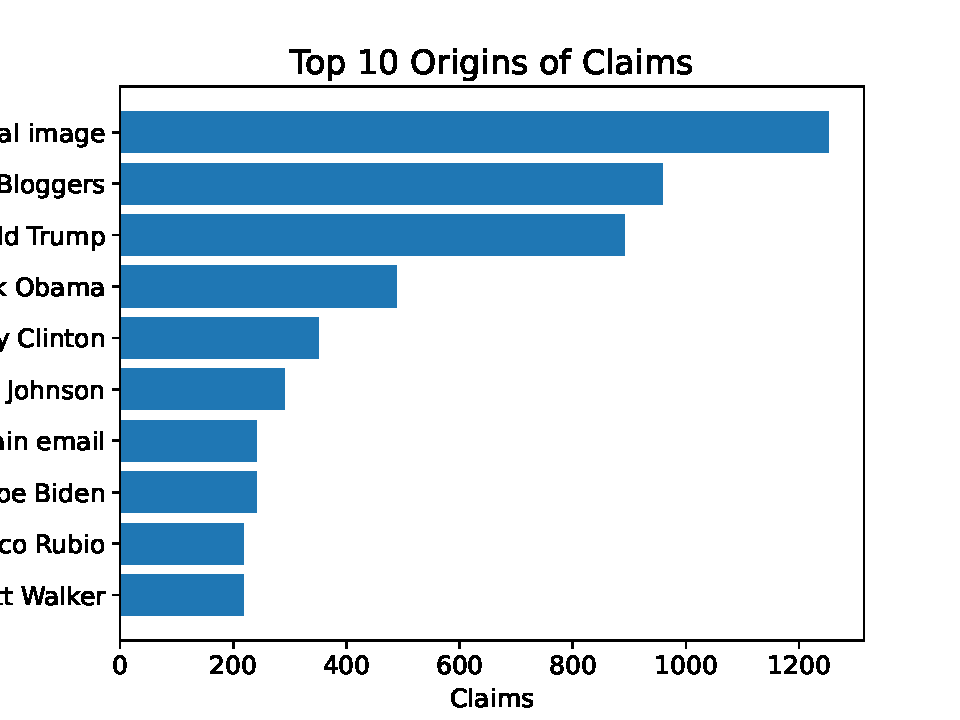
\includegraphics[width=6cm]{plots/origin_pltfct.pdf}}
    \qquad
    \subfloat[Top 10 topics in claims\label{fig:pltfct_topics}]{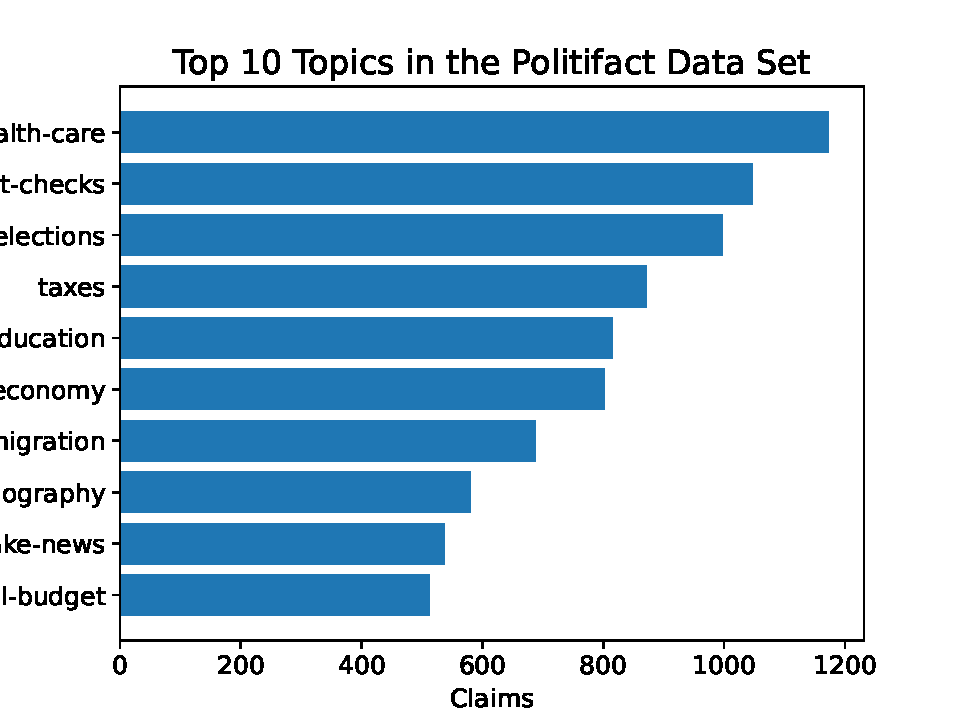
\includegraphics[width=6cm]{plots/topics_pltfct.pdf}}
    
    \subfloat[Cummulative number of claims over time\label{fig:pltfct_time}]{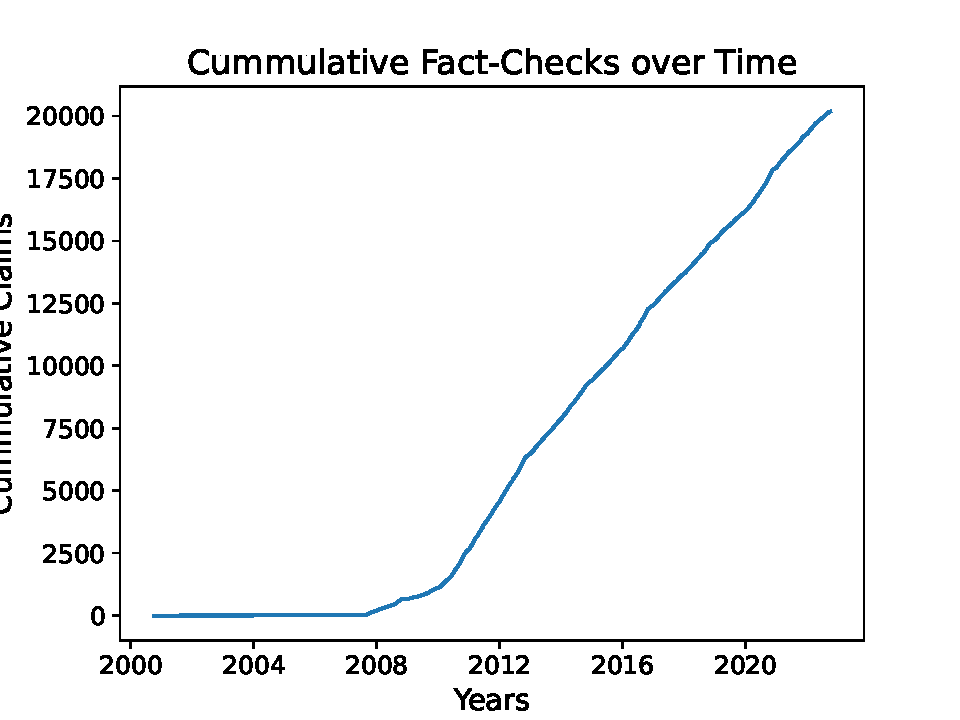
\includegraphics[width=6cm]{plots/time_pltfct.pdf}}
    \qquad
    \subfloat[Distribution of truth values in claims\label{fig:pltfct_truth_o_meter}]{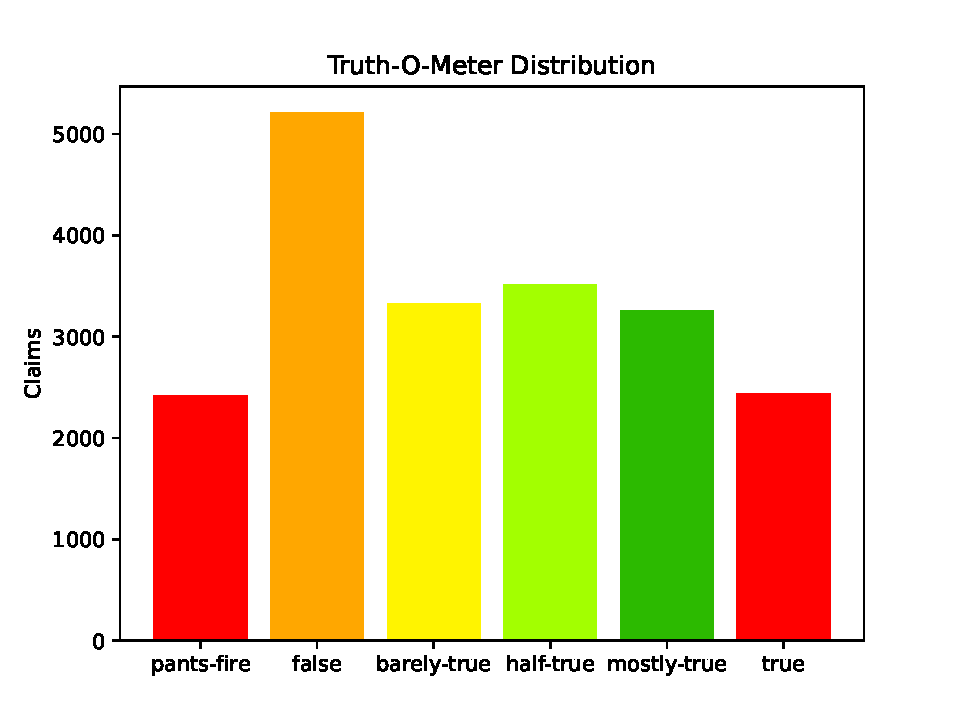
\includegraphics[width=6cm]{plots/truth-o-meter_distr.pdf}}

    \caption{General data characteristics of the fact-checked data set of claims derived from Politifact.}
    \label{fig:pltfct_subplots}
    
\end{figure}




% TABLES
\label{app_linear_data_upsample}
%table example
\begin{table}[H]
  \tiny %15
  \begin{center}
  \begin{tabular}{llllllll}
\toprule
{} &                         claim &                   origin &         url &  truth\_value &           stated\_on &           topic &         party \\
index &                               &                          &             &              &                     &                 &               \\
\midrule
29775 &  Thanks to the Act 10 coll... &  Wisconsin State AFL-CIO &  https:/... &  barely-true &        June 2, 2015 &           labor &  Organization \\
34391 &  "Wrong" COVID-19 case cou... &           Michael Caputo &  https:/... &        false &       July 14, 2020 &   public-health &    Republican \\
16341 &  "I committed to public fi... &             Barack Obama &  https:/... &  mostly-true &   February 20, 2008 &          ethics &      Democrat \\
3177  &  Wagon arriving at Detroit... &                 Bloggers &  https:/... &        false &    November 4, 2020 &       elections &          None \\
3025  &  “There were several state... &             Charlie Kirk &  https:/... &  barely-true &     January 7, 2021 &       elections &    Republican \\
33978 &  The health care bill "dum... &            Mike Huckabee &  https:/... &    half-true &   February 25, 2010 &         poverty &    Republican \\
38080 &  "The average state pensio... &        Rebecca Kleefisch &  https:/... &    half-true &     August 31, 2011 &    state-budget &    Republican \\
21452 &  "Barack Obama asked Ukrai... &             Donald Trump &  https:/... &  barely-true &  September 29, 2019 &  foreign-policy &    Republican \\
38608 &  "Texas has 600,000 regist... &             John Skvarla &  https:/... &  mostly-true &      April 14, 2016 &          states &    Republican \\
39614 &  "For the last 10 years, o... &              John Larson &  https:/... &    half-true &    October 22, 2017 &           taxes &      Democrat \\
\bottomrule
\end{tabular}

  \caption{Sample from our complete Politifact fact-checked news data set consisting of \pltfctTOTAL\ claims. The index contains the original index prior to any pre-processing steps. "claim" contains the actual news claim. "origin" is representing the origin of the claim (e.g., the claimant). "url" contains the Politifact subpage describing the claim and assessment of it. "truth\_value" is the Politifact truth evaluation of the claim. "stated\_on" shows the date of the claim. "party" shows the political affiliation of the claimant if any.}
  \label{tbl:politifact}
  \end{center}
\end{table}

Politifact summarizes every evaluated fact-check in one sentence. We store the fact-checked claims as \texttt{claim} in the \texttt{politifact\_claims.csv} available in the \texttt{fugazi-project} repository\footnote{Available on https://github.com/lrnz-asnprs/tweet-collector}, and as shown in data sample in table \ref{tbl:politifact}. The Politifact claims often either comprise 1) a statement or quote by the claimant (e.g., "There were no guns whatsoever at the Capitol riot on Jan. 6." - Donald Trump), 2) a summarizing paraphrasing of a piece of (fake) news (e.g., "Queen Elizabeth died because of the COVID-19 vaccine." - tweet), 3) or the original headline of a piece of (fake) news (e.g., "The U.S. & Elon Musk Reveal New Hypersonic Jet To Help Ukraine" - blogger). The average length of the fake news claim on Politifact is \pltfctMEANCLAIMLENCHARACTERS\ characters of length. The preliminary indexes of the claims (i.e., prior to any pre-processing steps being applied) are kept in place to ensure traceability throughout the research process. This is the indexing, we use to navigate claims in later proceedings in sections \ref{sec:tweet_collection}. Every claim has the date representing the date when the claim first was stated or started spreading online. As first introduced in section \ref{subsec:politifact}, all claims are assigned a value spanning from pants-on-fire to true. Table \ref{tbl:politifact} presents a sample from our data set.


% Add details about how claims often are summaries of the actual quotes and claims. A lot of them stem from direct claims:
% Examples where it becomes paraphrasings: 
% Also highlight to what extend the content consists of 
% https://www.politifact.com/factchecks/2013/apr/19/associated-industries-florida/associated-industries-florida-says-insurance-tax-c/
% 





\section{Tweet collection}
\label{sec:tweet_collection}

% Jaccard Similarity of Duplicated Tweets

\subsection{Collecting fake news on Twitter}

% BOT DETECTION METHODOLOGY LIMITATION --> REFERENCE THE BETTER APPROACH OF GRINBERG  Grinberg intelligently sampled his set of 16,442, by mapping U.S. voter registrations to twitter accounts to ensure getting real people. BOTNOT is also another better option.

% -- Collecting Fake News Claims on Twitter
% 2. Fetching Fake News shared on Twitter 
%   - Twitter API and setup
%   - Scripts to fetch verified fake-news
%   - Filtering for stopwords and Twitter API formatting
%   - Filtering for stopwords -- the precise approach should be left for an appendix!
%   - Presenting some general characteristics of the data
% 6. HPC and running the code in the cloud (timeline for the data collection)
% 7. Collecting Recent Tweets Following Data

\section{User Selection}

With our tweet collection procedure, we were able to identify an extensive amount of user profiles that were engaged in sharing of misinformation. In total, we collected 1.550.325 user profiles.

% 3. User bucketing and aggregate falsity scores
%   - Fake/True Users
%   - Filtering for non-human accounts (more than 25 tweets per day etc.)
%   - Quality insurance --> Only taking users that have at least 10 shares of fake news. 
%   - Aggregate falsity scores - The calculation --> derived from the label of Politifact


% Discuss current state-of-the-art approaches 
% Reason why we went for our specific approach

\section{A Holistic Framework To Quantify Drivers of Misinformation Belief} 

\subsection{Worldview}

% Evaluation of current approaches and reasoning
% - 
% ADD the Osmund stuff with regards --> They 250 --> we have 260. Say that we combine the two in our approach.

Although \cite{osmundsen2021partisan} determines political orientation through survey results, they also use source-based political  news outlets to determine.


% Description of our approach
% - 



% Maybe differentiate between congruent and incongruent

\subsection{Source cues}

% Reasoning why we chose to do so

% Evaluation of current approaches and reasoning



We describe the quantification approaches for elite exposure and in-group effect. 

\subsubsection{Elite exposure} \label{sec:elite_exposure}

% Reasoning why we chose to do so

Misleading claims by experts and political elites can be particularly damaging, because the trust in those with power can cause a shift of public opinion \citep{brulle2012shifting}. In order to examine the effect of elite exposure, we utilize a list of Twitter accounts of 816 political elites associated with an average falsity score \citep{mosleh2021elites}. Employing this approach allows us to overcome a key methodological challenge of social media studies, namely estimating which content a Twitter user is likely consuming or exposed to. Clearly, the accounts that a user follows are only a proxy for what users would consume on Twitter \citep{mosleh2021elites}.

We calculate the elite driver effect of the users in our dataset by taking the weighted average of the falsity scores of the elites they are following. The weights of each elite account are determined by the average number of tweets per two-month period in the past two years, which serves as a proxy for intensity of exposure \citep{mosleh2021elites}. 

\subsubsection{In-group effect}

% Reasoning why we chose to do so

To quantify the in-group effect, we use a similar methodology as for elite exposure in section \ref{sec:elite_exposure}. Here, we compute the weighted average falsity score of in-group members of a Twitter user. We define as in-group members, all mutual friends of a user. I.e., a user where there exists a reciprocal connection: user A follows user B and user B follows also user A. The weights are determined by the average amount of tweets of a user in a two-month period. 

% Analysis:

%We compare both average elite exposure scores as well as in-group scores to the average of the set of true users to test if these scores are significantly different.

%We visualize the elite exposure scores and in-group scores in a following network.

\subsection{Emotion} \label{sec:emotion_quantification}

% Reasoning why we chose to do so

% Evaluation of current approaches and reasoning
% Description of our approach



To extract emotional features of users in our dataset, we base our method on the work of \cite{karami2021profiling}. We treat each user as a document and the users' recent tweets are considered as the content of that document. For quantifying the emotional features we exploit the Linguistic Inquiry and Word Count (LIWC) dictionary \citep{tausczik2010psychological}. We measure the features by calculating the percentage of words in a users recent tweets that belong to each category. In the following, we list the extracted categories from LIWC.

\begin{itemize}
    \item In LIWC there are several general \textit{emotional} categories present. First, positive emotion (\textit{emo pos}) with words such as good, love, happy, hope. Second, negative emotion (\textit{emo neg}) with words like bad, hate, hurt, tired. Third, anger (\textit{emo anger}) expressed by e.g., hate, mad, angry. Lastly, we selected sadness \textit{emo sad}, given by words like sad, disappoint*, cry.
    \item We selected two LIWC features related to \textit{uncertainty}. First, discrepancy (e.g., should, would, could) and second, \textit{tentativeness} (e.g., maybe, perhaps, guess).
    \item Further, we measure \textit{anxiety} with the LIWC Anxiety category that includes words like nervous, afraid, and tense.
    \item Lastly, we measure \textit{lack of control} by the LIWC category \textit{futurefocus}. This feature includes words like will, going to, have to, may.
\end{itemize}


% We perform two experiments towards this goal. First, we set our null hypothesis to be that these two groups have the same mean in five categories of features. If the results of t-test shows that there is a significant difference (p-value less than 0.05) between two groups, we can reject the null hypothesis

\subsection{Illusory Truth}

% Reasoning why we chose to do so

% Evaluation of current approaches and reasoning

% Description of our approach
\subsubsection{Familiarity}


% MOTIVATION/RATIONALE

The effect of repeated exposure to stimuli on ones perception of truth has been replicated many times and has been found to be a robust phenomenon \citep{dechene2010truth}. 

Although most studies examining the illusory truth effect have used three or fewer repetitions. Some scholars investigated the effect with multiple repetitions \citep{koch2013helpful, difonzo2016validity, hassan2021effects}. \cite{hassan2021effects} have found that perceived truthfulness increased logarithmically with the number of exposures. They conducted two experiments where participants were presented with trivia statements up to 9 and 27 times respectively. According to their findings, the largest effect on perceived truth appeared after the second exposure and was marginally smaller with additional repetitions.

----

% APPROACH

Our approach to quantify the familiarity effect is based on estimating a user's news feed from the tweets posted by their followees. Analogous to \cite{grinberg2019partisanship}, we define tweets to which a user was potentially exposed to, their "exposures". In order to measure the effect of prior exposure to a misinformation, we link back each labeled tweet (FT) on a user's news feed to its originating fact-checked claim (C). We focus on those claims made by a users with a detectable familiarity effect ($C_i$). I.e., those claims, to which a user has been exposed to before. Using the timestamps of the tweets, we are able to reconstruct prior exposures to claims. We label each claim $C_i$ as $C_i_j$, where $j$ refers to a prior exposure to this claim. We then compute the logarithm of the count of prior exposure to such claim, to account for diminishing effects as suggested by \cite{hassan2021effects}. Finally, we normalize the sum of all prior exposures by the amount of claims with detectable effects. We do so to avoid inflating the effect simply because a user is tweeting a lot.


\[familiarity-effect = \frac{\displaystyle \sum_{n=1}^{i}\log_{e}(\sum_{n=1}^{j}C_i_j)}{|C_i|}\]


\subsubsection{Fluency}

To measure the \emph{fluency} of a claim, we focus primarily on the readability of the claim. Although, there exist numerous approaches of assessing the readability of texts, we chose to employ two of the most established approaches. First, the Flesch reading-ease score \citep{flesch1948new} and second, the Dale-Chall Readability Formula \citep{dale1948formula, chall1995readability}. 

The Flesch formula scores a text between 1 and 100, with 100 being the easiest to read. The score incorporates both the sentence complexity (words per sentence) as well as the word complexity (syllables per words). Due to it's simplicity it has become a standard baseline for readability assessment. 

\[ 206.835 - 1.015 (\frac{\emph{words}}{\emph{sentences}}) - 84.6 (\frac{\emph{syllables}}{\emph{words}}) \]

The Dale-Chall readability measure shows that the ratio of difficult words in a text and the number of words per sentence determine the comprehensibility of a text. Based on the formula, every word is considered to be difficult, that is not contained on a list of 3.000 words a fourth-grade American student should be familiar with. Unlike the Flesch formula, the Dale-Chall scores are reported on a scale from < 4.9 to 9.9, where the lower end of the scale refers to easier understandable texts.

\[ 0.1579 (\frac{\emph{difficult words}}{\emph{words}}) + 0.0496 (\frac{\emph{words}}{\emph{sentences}}) \]

Most traditional readability formulas like the Flesch or Dale-Chall score are considered valid for text samples with a significant sample size of text and are therefore not necessarily suitable for a tweet text of short length. Prior research modified the Flesch formula by treating tweets as single sentences, because of their character limit, use of hashtags and non-traditional punctuation \citep{collins2014computational}. This research has been conducted however, during a time when tweets had a character limit of 140, and may become inadequate for the recent character limit of 280. Hence, we chose apply the traditional Flesch Reading Ease formula in this initial study, building upon existing research that has examined the readability of tweets by employing the conventional readability formula on tweets \citep{jacob2019readability}. We validate our results by calculating the Pearson and Spearman correlations between the Flesch and Dale-Chall score. Both the Pearson ($r = -.73$, $p<.001$) as well as the Spearman correlation coefficients ($r = -.74$, $p<.001$) report a negative correlation between the two scores. A negative correlation is desirable, as a high Flesch score indicates easier readability, whereas the opposite applies to the Dale-Chall formula. 

\begin{figure}[H]
    \centering
    
    \subfloat[Top 10 origins of claims\label{fig:pltfct_origin}]{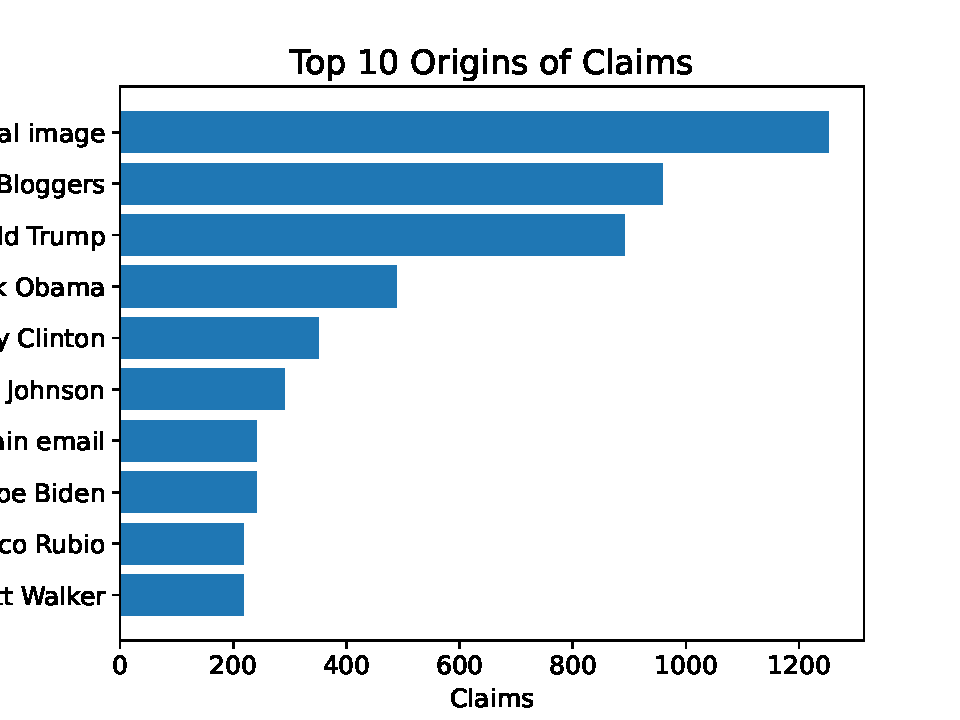
\includegraphics[width=6cm]{plots/origin_pltfct.pdf}}
    \qquad
    \subfloat[Top 10 topics in claims\label{fig:pltfct_topics}]{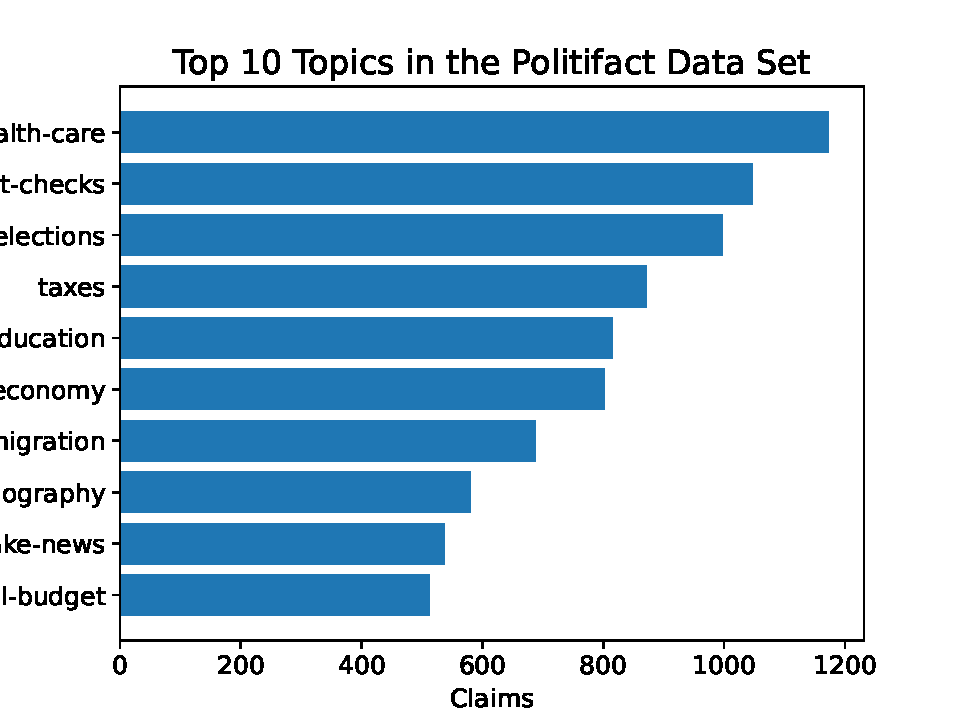
\includegraphics[width=6cm]{plots/topics_pltfct.pdf}}
    
    \subfloat[Cummulative number of claims over time\label{fig:pltfct_time}]{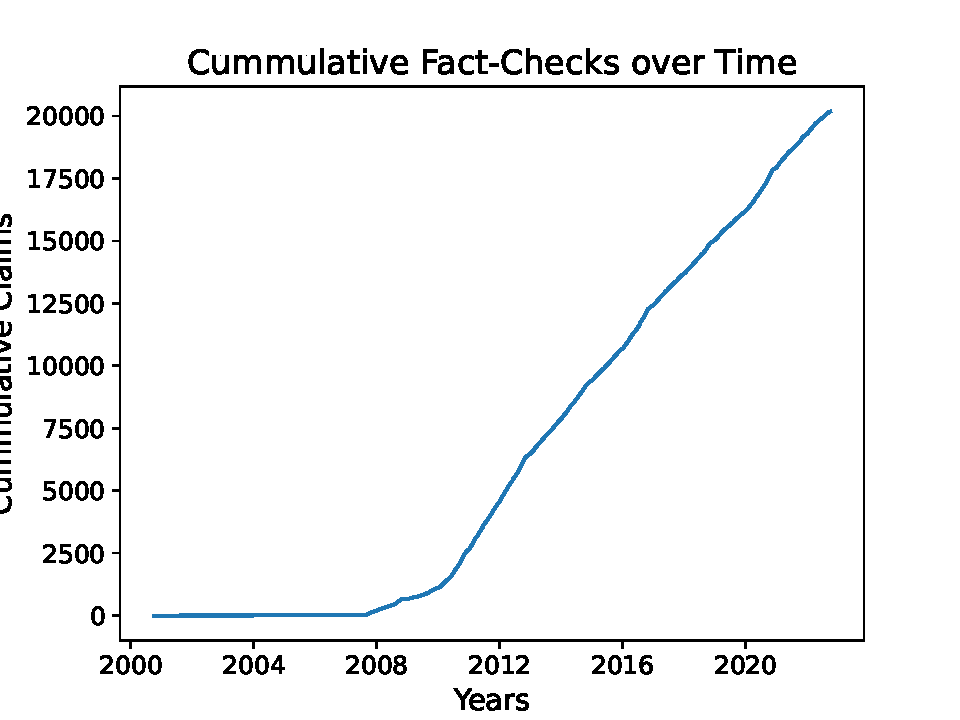
\includegraphics[width=6cm]{plots/time_pltfct.pdf}}
    \qquad
    \subfloat[Distribution of truth values in claims\label{fig:pltfct_truth_o_meter}]{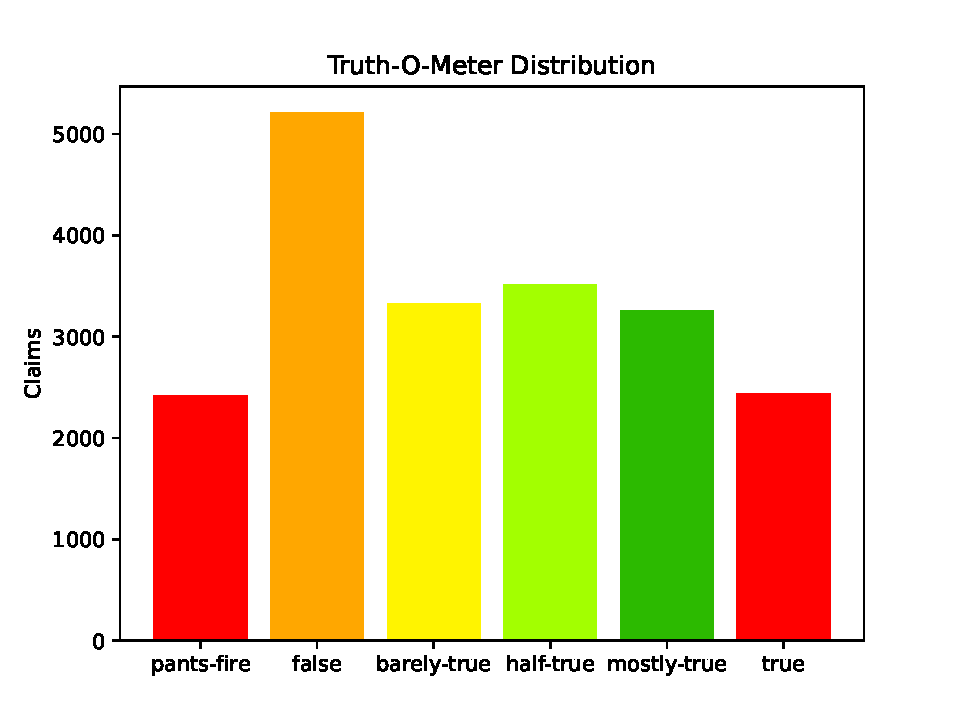
\includegraphics[width=6cm]{plots/truth-o-meter_distr.pdf}}

    \caption{General data characteristics of the fact-checked data set of claims derived from Politifact.}
    \label{fig:pltfct_subplots}
    
\end{figure}

We compute the impact of the \emph{fluency} driver as the average Flesch score of all claims shared by a user. This metric should serve as a proxy of how comprehensible the claims processed by a user were on average. 

%Computational Assessment of Text Readability: A Survey of Current and Future Research
%While traditional readability formulas like Flesch-Kincaid are widely-available and relatively easy to compute, they also have some serious limitations, especially in the context of the Web and online information access. First, such formulas make strong  assumptions about the text being assessed: They typically assume the text has no noise, or limited noise, and that it consists of well-formed sentences. Second, traditional measures also require significant sample sizes of text, since they become unreliable for passages with less than 300 words (cf. Kidwell et al., 2009). Third, a number of recent studies have demonstrated the unreliability of traditional readability measures for Web pages and other types of non-traditional documents (Si and Callan, 2001; CollinsThompson and Callan, 2004; Peterson and Ostendorf, 2006; Feng et al., 2009). 


\subsection{Intuitive Thinking}

% Reasoning why we chose to do so

% Evaluation of current approaches and reasoning
% Description of our approach

To quantify the extent to which an individual user is engaged in analytical or intuitive thinking, we exploit the LIWC category \emph{Analytic}. This feature quantifies the degree of analytical and logical thinking, as opposed to more intuitive writing. This category is determined by prior research linking the use of articles to logical and analytical thinking \citep{pennebaker2014small}. The LIWC Analytic feature is reported as a standardized variable transformed to a scale from 1 to 100.

\chapter{Results} \label{results}

\section{Assessment Of Drivers Individually}

% Comparison and Analysis ideas:

% - Summary statistics for users in each subgroup (see SM paper fake news during presidential elections 2016 page 36)

% - Plot probability distribution of exposure to false claims from friends for each group (low agg fals -> high agg fals) like in this paper: https://sel.sise.bgu.ac.il/assets/pubs/fake-news-science-2019.pdf

% - Plot distribution of political idealogy for each group (low fals score - high fals score)

% - T-tests for differences in agg emotions between groups

% - Verify accuracy of approach of labeling political orientation based on news sources shared with following of politicans 



\section{Assessment of Drivers Combined}

- Here we describe the feature importance analysis of our aggregated model.
- We show the impact of different combinations of drivers and user features

What can we do to improve the quality of the analysis?

Correlation matrix for the features

\chapter{Discussion}
\label{conclusion}







%----------------------------------------------------------------------------------------
%	BIBLIOGRAPHY
%----------------------------------------------------------------------------------------

\bibliographystyle{chicago} 
\bibliography{thesisbiblio}
\addcontentsline{toc}{chapter}{Bibliography}


%----------------------------------------------------------------------------------------
%	APPENDICES
%----------------------------------------------------------------------------------------
\newpage
\appendix
\chapter{Appendix}
\label{appendices}

\section{Figures}
\label{app:figures}
%FIGURES

\subsection{Politifact webpage}
\begin{figure}[H]
    \centering
    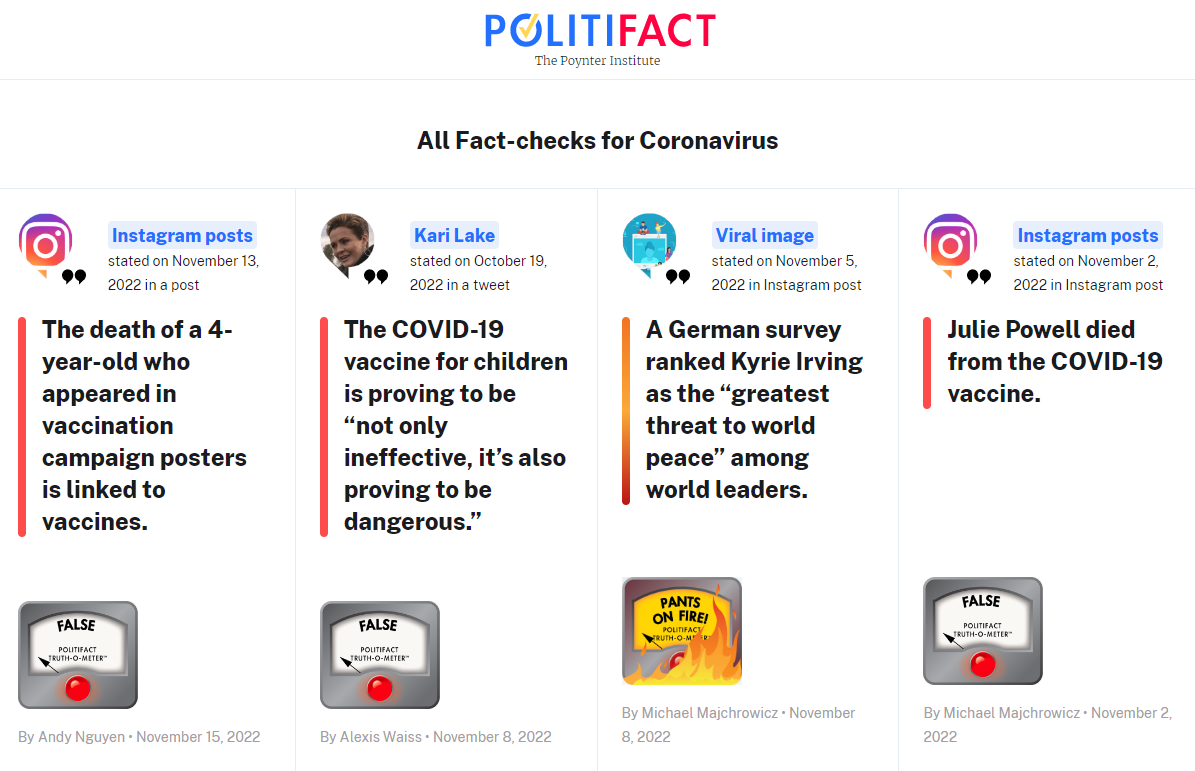
\includegraphics[width=20cm,height=8cm,keepaspectratio]{figures/politifact22112022.png}
    
    \caption{Screenshot of politifact.com looking under fact checks related to Coronavirus}
    \label{fig:politifact_page_content}
\end{figure}



\clearpage
\section{Tables}
\label{app:tables}


\section{Code}
\label{app:code}



\end{document}



